\documentclass[tikz,border=2pt]{standalone}
\usepackage{amsmath,amssymb}
\usetikzlibrary{arrows.meta}
\begin{document}
% Ex 4.6.6: arrivals at 0,2,4,6, service 1, one server. L = 1 on [2k,2k+1), 0 on [2k+1,2k+2).
% Half the time in each state; all arrivals see state 0: lambda(0) = 1, lambda(1) = 0,
% lambda = 1/2 = lambda(0) p(0) + lambda(1) p(1).
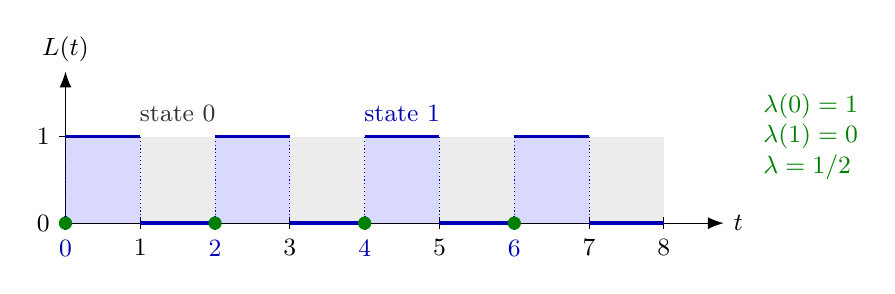
\begin{tikzpicture}[font=\small, >={Latex[length=2mm]}, x=0.95cm, y=1.1cm]
  % time in state 0 (gray bands) and in state 1 (blue under the path)
  \foreach \a in {1,3,5,7} {\fill[gray!15] (\a,0) rectangle (\a+1,1);}
  \foreach \a in {0,2,4,6} {\fill[blue!15] (\a,0) rectangle (\a+1,1);}
  % axes
  \draw[->] (0,0) -- (8.8,0) node[right] {$t$};
  \draw[->] (0,0) -- (0,1.75) node[above] {$L(t)$};
  \draw (0.08,1) -- (-0.08,1) node[left] {$1$};
  \node[left] at (-0.08,0) {$0$};
  \foreach \x in {1,3,5,7,8} {\draw (\x,0.07) -- (\x,-0.07) node[below] {$\x$};}
  % path
  \foreach \a in {0,2,4,6}
    {\draw[blue!70!black, very thick] (\a,1) -- (\a+1,1);
     \draw[blue!70!black, very thick] (\a+1,0) -- (\a+2,0);
     \draw[blue!70!black, thin, densely dotted] (\a,0) -- (\a,1);
     \draw[blue!70!black, thin, densely dotted] (\a+1,0) -- (\a+1,1);}
  % arrivals and what they see
  \foreach \a in {0,2,4,6}
    {\draw[blue!70!black, thick] (\a,0.08) -- (\a,-0.08) node[below] {$\a$};
     \fill[green!50!black] (\a,0) circle (2.4pt);}
  % labels of the two states
  \node[gray!40!black, anchor=south] at (1.5,1.06) {state $0$};
  \node[blue!70!black, anchor=south] at (4.5,1.06) {state $1$};
  % rates
  \node[green!50!black, anchor=west, align=left] at (9.2,1.0)
    {$\lambda(0)=1$\\ $\lambda(1)=0$\\ $\lambda=1/2$};
\end{tikzpicture}
\end{document}
